%%%%%%%%%%%%%%%%%%%%%%%%%%%%%%%%%%%%%%%%%
% Focus Beamer Presentation
% LaTeX Template
% Version 1.0 (8/8/18)
%
% This template has been downloaded from:
% http://www.LaTeXTemplates.com
%
% Original author:
% Pasquale Africa (https://github.com/elauksap/focus-beamertheme) with modifications by 
% Vel (vel@LaTeXTemplates.com)
%
% Template license:
% GNU GPL v3.0 License
%
% Important note:
% The bibliography/references need to be compiled with bibtex.
%
%%%%%%%%%%%%%%%%%%%%%%%%%%%%%%%%%%%%%%%%%

%----------------------------------------------------------------------------------------
%	PACKAGES AND OTHER DOCUMENT CONFIGURATIONS
%----------------------------------------------------------------------------------------

\documentclass{beamer}

\usetheme{focus} % Use the Focus theme supplied with the template
% Add option [numbering=none] to disable the footer progress bar
% Add option [numbering=fullbar] to show the footer progress bar as always full with a slide count

% Uncomment to enable the ice-blue theme
%\definecolor{main}{RGB}{92, 138, 168}
%\definecolor{background}{RGB}{240, 247, 255}

%------------------------------------------------

\usepackage{booktabs} % Required for better table rules

%----------------------------------------------------------------------------------------
%	 TITLE SLIDE
%----------------------------------------------------------------------------------------

\title{Focus: \\ INTERIOR-POINT METHODS}

%\subtitle{Subtitle}

\author{\small  Jean KOUAGOU\\ Ariel KEMOGNE \\ Blessing BASSEY \\ Gedeon MUHAWENAYO}

\titlegraphic{
\includegraphics[scale=0.3]{Images/logo.jpeg}} % Optional title page image, comment this line to remove it

\institute{African Masters for Machine Learning}% \\ Institute Address}

\date{13 12 2019}

%------------------------------------------------


\begin{document}

%------------------------------------------------
\tableofcontents
\begin{frame}
	\maketitle % Automatically created using the information in the commands above
\end{frame}

%----------------------------------------------------------------------------------------
%	 SECTION 1
%----------------------------------------------------------------------------------------

%\section{Introduction} % Section title slide, unnumbered

%\begin{frame}{Columns}
%	\begin{columns}
%		\column{0.5\textwidth}
%			It is
%			widely accepted nowadays that there exist classes of problems for which one
%			method may significantly outperform the other. The large size of the problem
%			generally seems to favour interior point methods. 
%		
%		\column{0.5\textwidth}
%			\includegraphics[width=\linewidth]{Images/Do you know.jpg}
%	\end{columns}
%\end{frame}
	

\begin{frame}{Introduction}
	\begin{columns}
		\column{0.5\textwidth}
			It is widely accepted nowadays that there exist classes of problems for which one method may \alert{significantly outperform} the other. The large size of the problem generally seems to favour interior point methods. 
		
		\column{0.5\textwidth}
			
\includegraphics[width=\linewidth]{Images/DO.jpeg}
	\end{columns}
\end{frame}





\begin{frame}{why interior point method}
An \alert {interior point method } is a linear or nonlinear programming method that achieves optimization by going through the \alert{middle} of the solid defined by the problem rather than its outer surface.
		\begin{figure}
		\centering
		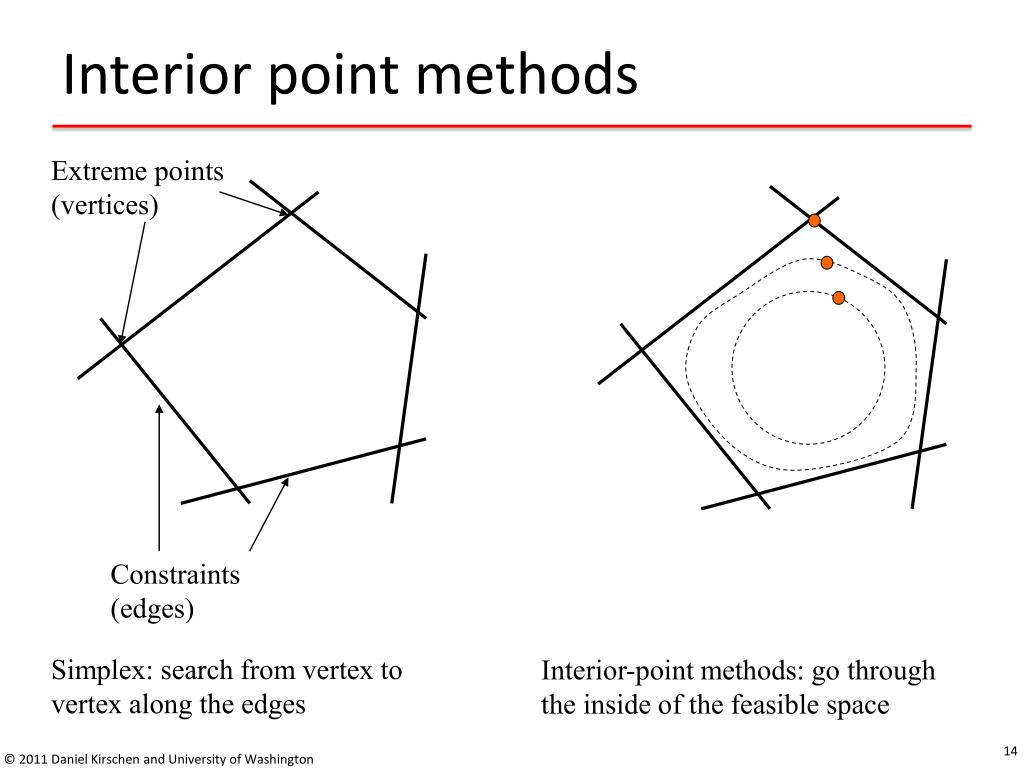
\includegraphics[width=0.6\linewidth]{Images/interior-point-methods-l}
		\caption{Simplex versus interior point method}
		%\label{fig:interior-point-methods-l}
	\end{figure}
	
\end{frame}

%------------------------------------------------

\begin{frame}[noframenumbering]{Inequality constrained minimization}
	\begin{equation*}
	\begin{array}{cl}\alert{\textbf{ Inequality constrained minimization }} \\[0.4cm] \textcolor{example}{\text { minimize }} & {f_{0}(x)} \\ \textcolor{example}{\text { subject to}} & {f_{i}(x) \leq 0, \quad i=1, \ldots, m} \\ & {A x=b}\end{array}
	\end{equation*}
	\begin{itemize}
		\item $f_i$ convex, twice continuously differentiable \\
		 \item A $ \in \mathbf{R}^{p \times n} $ with rank $ A = p$ \\
		 \item we assume  $ p^{\star} $  is finite and attained \\
		 \item  we assume problem is strictly feasible: there exists $ \tilde{x}$ with $ \tilde{x} \in \operatorname{dom} f_{0},\ f_{i}  (\tilde{x})<0, \quad i=1, \ldots, m$,\ $A\tilde{x}=b$
		  hence, strong duality holds and dual optimum is attained.
	\end{itemize}
\end{frame}

%------------------------------------------------

\begin{frame}[noframenumbering]{Logarithmic barrier}
	\alert{Approximation with the indicator function}
	\begin{equation*}
	\begin{array}{ll}{\text { minimize }} & {f_{0}(x)+\sum_{i=1}^{m} I_{-}\left(f_{i}(x)\right)} \\ {\text { subject to }} & {A x=b}\end{array}
	\end{equation*}
where
	$I_{-}(u)=0 \text { if } u \leq 0, I_{-}(u)=\infty
	$ otherwise.\\ [0.4cm]
	\alert{Approximation via logarithmic barrier}
	\begin{equation*}
	\begin{array}{ll}{\text { minimize }} & {f_{0}(x)-(1 / t) \sum_{i=1}^{m} \log \left(-f_{i}(x)\right)} \\ {\text { subject to }} & {A x=b}\end{array}
	\end{equation*}
\end{frame}
%------------------------------------------------

\begin{frame}[noframenumbering]{Logarithmic barrier function}
	\begin{equation*}
	\phi(x)=-\sum_{i=1}^{m} \log \left(-f_{i}(x)\right), \quad \operatorname{dom} \phi=\left\{x | f_{1}(x)<0, \ldots, f_{m}(x)<0\right\}
	\end{equation*}
	\begin{equation*}
	\begin{array}{l}{\bullet \text { convex (follows from composition rules) }} \\ {\bullet \text { twice continuously differentiable, with derivatives }}\end{array}
	\end{equation*}
	\begin{equation*}
	\begin{aligned} \nabla \phi(x) &=\sum_{i=1}^{m} \frac{1}{-f_{i}(x)} \nabla f_{i}(x) \\ \nabla^{2} \phi(x) &=\sum_{i=1}^{m} \frac{1}{f_{i}(x)^{2}} \nabla f_{i}(x) \nabla f_{i}(x)^{T}+\sum_{i=1}^{m} \frac{1}{-f_{i}(x)} \nabla^{2} f_{i}(x) \end{aligned}
	\end{equation*}
\end{frame}

\begin{frame}[noframenumbering]{Central path}
\begin{equation*}
\begin{aligned} \bullet \text { for } t>0, \text { define } x^{\star}(t) \text { as the solution of } \\ \qquad \begin{array}{ll}{\text { minimize }} & {t f_{0}(x)+\phi(x)} \\ {\text { subject to }} & {A x=b}\end{array} \end{aligned}
\end{equation*}

 (for now, assume $ x^{\star}(t) \text { exists and is unique for each } t>0 \text { ) }
$
 
~~~~~~~~~~~~~~~~~~~~$\bullet$  the central path is $\left\{x^{\star}(t) | t>0\right\}
$
\end{frame}
%------------------------------------------------
\begin{frame}[noframenumbering]{Dual points on central path}
\begin{equation*}
\begin{aligned} \\\alert {x=x^{\star}(t) \text { if there exists a } \textcolor{example}{w} \text { such that }} \\ \qquad t \nabla f_{0}(x)+\sum_{i=1}^{m} \frac{1}{-f_{i}(x)} \nabla f_{i}(x)+A^{T} w=0, & \qquad A x=b \end{aligned}
\end{equation*}

\begin{equation*}
\bullet \text { therefore, } x^{\star}(t) \text { minimizes the Lagrangian }
\end{equation*}
\begin{equation}
L\left(x, \lambda^{\star}(t), \nu^{\star}(t)\right)=f_{0}(x)+\sum_{i=1}^{m} \lambda_{i}^{\star}(t) f_{i}(x)+\nu^{\star}(t)^{T}(A x-b)
\end{equation}
\begin{equation*}
\text { where we define } \lambda_{i}^{\star}(t)=1 /\left(-t f_{i}\left(x^{\star}(t)\right) \text { and } \nu^{\star}(t)=w / t\right.
\end{equation*}
\end{frame}


\begin{frame}[noframenumbering]{Interpretations via KKT Conditions}
\begin{equation*}
\begin{array}{l} \alert{x=x^{\star}(t), \lambda=\lambda^{\star}(t), \nu=\nu^{\star}(t) \text { satisfy }} \\ {\text { 1. primal constraints: } f_{i}(x) \leq 0, i=1, \ldots, m, A x=b} \\ {\text { 2. dual constraints: } \lambda \succeq 0} \\ {\text { 3. approximate slackness: }
-\lambda_{i} f_{i}(x)=1 / t, i=1, \ldots, m} \\ {\text { 4. gradient of Lagrangian with respect to } x \text { vanishes: }}\end{array}
\end{equation*}
\begin{equation*}
\nabla f_{0}(x)+\sum_{i=1}^{m} \lambda_{i} \nabla f_{i}(x)+A^{T} \nu=0
\end{equation*}
\begin{equation*}
\text { The difference with } \mathrm{KKT} \text { is that condition } 3 \text { replaces } \lambda_{i} f_{i}(x)=0
\end{equation*}
\end{frame}


\begin{frame}[noframenumbering]{Barrier Method}
\begin{equation*}
\begin{array}{l}{\text { Given strictly feasible } \textcolor{example}{x, t:=t^{(0)}>0, \mu>1,} \text { tolerance } \textcolor{example}{\epsilon>0}} \\ \alert{\text { repeat }} \\ {\text { 1. Compute } x^{\star}(t) \text { by minimizing } t f_{0}+\phi, \text { subject to } A x=b} \\ {\text { 2. Update. } x:=x^{\star}(t)} \\ {\text { 3. Stopping criterion: quit if } m / t<\epsilon} \\ {\text { 4. Increase } t:\  t:=\mu t}\end{array}
\end{equation*}

\begin{itemize}
\item Terminates with $ f_{0}(x)-p^{\star} \leq \epsilon$
\item Centering usually done using Newton's method, starting at current $x$
\item Choice of $\mu$  involves a trade-off: $ \mu$ means fewer outer iterations
\item  More inner (Newton) iterations; typical values:  $\mu=10-20$ several heuristics for choice of $ t^{(0)}$
\end{itemize}
\end{frame}

\begin{frame}[noframenumbering]{Convergence Analysis}
\begin{equation*}
\begin{array}{l}{\text { Number of outer (centering) iterations: exactly }} \\ {\qquad\left[\frac{\log \left(m /\left(\epsilon t^{(0)}\right)\right)}{\log \mu}\right]} \\ { \text { plus the initial centering step (to compute }\left.x^{\star}\left(t^{(0)}\right)\right)}\end{array}
\end{equation*}
\begin{figure}
	\centering
	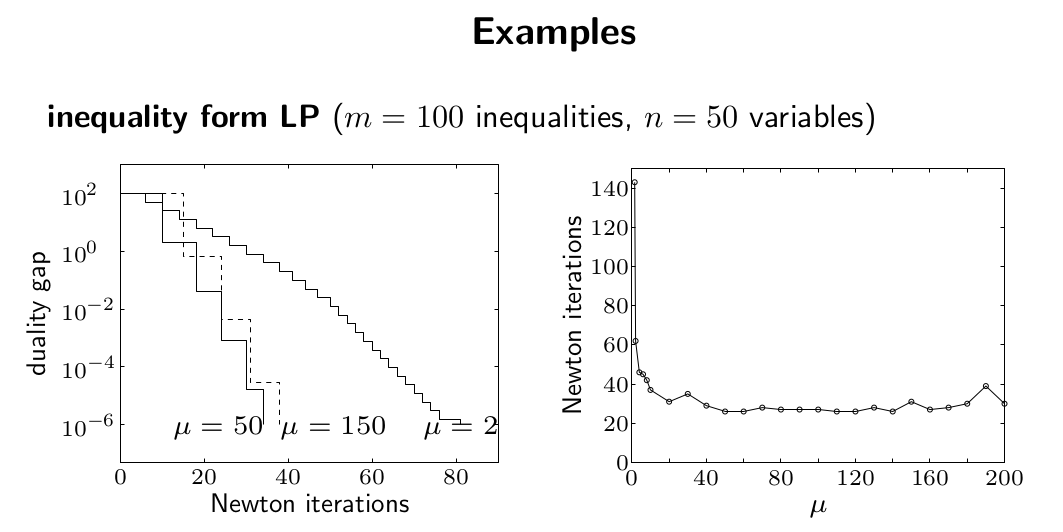
\includegraphics[width=0.7\linewidth]{Images/example}
	%\caption{}
	\label{fig:example}
\end{figure}
\end{frame}

\begin{frame}[noframenumbering]{Feasibility and phase I methods}
\begin{equation*}
\begin{array}{l} \\ \textcolor{example}{\text {{Feasibility problem:}}} \quad find \ x  \text { such that } \\ {\qquad f_{i}(x) \leq 0, \quad i=1, \ldots, m, \quad A x=b}\end{array}
\end{equation*}
\begin{equation*}
\begin{array}{l} {\text { \textbf{phase I}: computes strictly feasible starting point for barrier method }} \\\\ \alert{\text { {basic phase 1 method} }}\end{array}
\end{equation*}
\begin{equation}
\begin{array}{ll}{ \text { minimize (over }x, s)} & {s} \\ {\text { subject to }} & {f_{i}(x) \leq s, \quad i=1, \ldots, m} \\ {} & {A x=b}\end{array}
\end{equation}
\alert{{Sum of infeasibilites phase 1 method }}
\begin{equation}
\begin{array}{cl}{\operatorname{minimize}} & {\mathbf{1}^{T} s} \\ {\text { subject to }} & {s \succeq 0, \quad f_{i}(x) \leq s_{i}, \quad i=1, \ldots, m} \\ {} & {A x=b}\end{array}
\end{equation}
\end{frame}


\begin{frame}[noframenumbering]{Basic vs sum of infeasibilities and phase I methods}
\begin{figure}
	\centering
	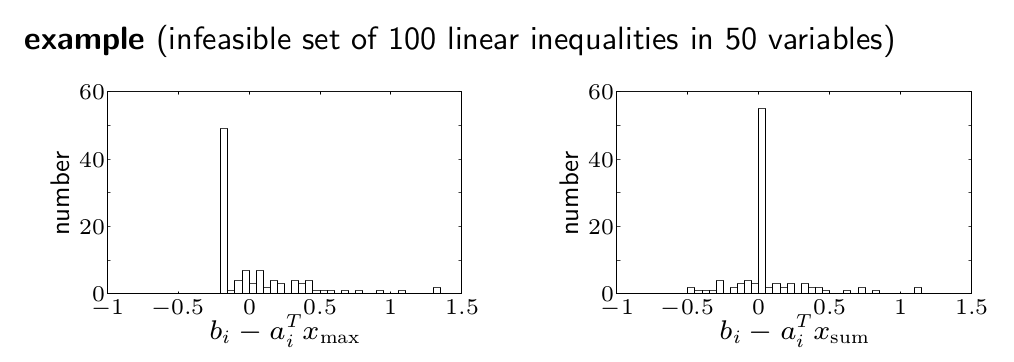
\includegraphics[width=1\linewidth]{Images/sum}
	%\caption{}
	%\label{fig:sum}
\end{figure}
\alert{Left graph} is the  basic phase I solution and it 39 inequalities,\\ \alert{Right graph}  is the sum of infeasibilities phase I solution satisfying 79 inequalities.
\end{frame}

\begin{frame}[noframenumbering]{Generalized inequalities}
\begin{equation*}  
\begin{array}{cl}\\ \textcolor{example}{\text { minimize }} & {f_{0}(x)} \\ \textcolor{example}{\text { subject to }} & {f_{i}(x) \preceq_{K_{i}} 0, \quad i=1, \ldots, m} \\ {} & {A x=b}\end{array}
\end{equation*}
\begin{equation*}
\begin{array}{l}{ \bullet \ f_{0} \text { convex, } f_{i}: \mathbf{R}^{n} \rightarrow \mathbf{R}^{k_{i}}, i=1, m, \text { convex with respect to proper }} \\ {\text { cones } K_{i} \in \mathbf{R}^{k_{i}}} \\\\ {\bullet \ f_{i} \text { twice continuously differentiable }} \\\\ {\bullet \ A \in \mathbf{R}^{p \times n} \text { with rank } A=p} \\\\ {\bullet\  \text {we assume problem is strictly feasible; hence strong duality holds and }} \\ {\text { dual optimum is attained }}\end{array}
\end{equation*}
\end{frame}

\begin{frame}[noframenumbering]{Generalized Logarithm for proper cone}
\begin{equation*}
\begin{array}{l}{\psi: \mathbf{R}^{q} \rightarrow \mathbf{R} \text { is generalized logarithm for proper cone } K \subseteq \mathbf{R}^{q} \text { if: }} \\ {\bullet \text { dom } \psi=\operatorname{int} K \text { and } \nabla^{2} \psi(y) \prec 0 \text { for } y \succ_{K} 0} \\ {\bullet \ \psi(s y)=\psi(y)+\theta \log s \text { for } y \succ_{K} 0, s>0(\theta \text { is the degree of } \psi)}\end{array}
\end{equation*}
\begin{equation*}
\begin{array}{l}\alert{\text { {Examples} }} \\ {\bullet \text { nonnegative orthant } K=\mathbf{R}_{+}^{n}: \psi(y)=\sum_{i=1}^{n} \log y_{i}, \text { with degree } \theta=n} \\ {\bullet \text { positive semidefinite cone } K=\mathbf{S}_{+}^{n}:}\end{array}
\end{equation*}
\begin{equation*}
\psi(Y)=\log \operatorname{det} Y \quad(\theta=n)
\end{equation*}
\begin{equation*}
\begin{array}{l}{\bullet \text { second-order cone } K=\left\{y \in \mathbf{R}^{n+1} |\left(y_{1}^{2}+\cdots+y_{n}^{2}\right)^{1 / 2} \leq y_{n+1}\right\}:} \\ {\quad \quad \psi(y)=\log \left(y_{n+1}^{2}-y_{1}^{2}-\cdots-y_{n}^{2}\right) \quad(\theta=2)}\end{array}
\end{equation*}
\end{frame}

\begin{frame}[noframenumbering]{Generalized logarithmic barrier and central paths}
	\begin{equation*}
	\alert{\text {Logarithmic barrier for }} f_{1}(x) \preceq_{K_{1}} 0, \ldots, f_{m}(x) \preceq_{K_{m}} 0
	\end{equation*}
	\begin{equation*}
	\phi(x)=-\sum_{i=1}^{m} \psi_{i}\left(-f_{i}(x)\right), \quad \text { dom } \phi=\left\{x | f_{i}(x) \prec_{K_{i}} 0, i=1, \ldots, m\right\}
	\end{equation*}
	\begin{equation*}
	\begin{array}{l}{\bullet \psi_{i} \text { is generalized logarithm for } K_{i}, \text { with degree } \theta_{i}} \\ {\bullet \phi \text { is convex, twice continuously differentiable }}\end{array}
	\end{equation*}
	\begin{equation*}
	\text { central path: }\left\{x^{\star}(t) | t>0\right\} \text { where } x^{\star}(t) \text { solves }
	\end{equation*}\\[0.2cm]
	\begin{equation*}
	\begin{array}{ll} \textcolor{example}{\text { minimize }} & {t f_{0}(x)+\phi(x)} \\ \textcolor{example}{\text { subject to }} & {A x=b}\end{array}
	\end{equation*}
	
\end{frame}



%
%\begin{frame}{Typesetting and Math}
%	The packages \texttt{inputenc} and \texttt{FiraSans}\footnote{\url{https://fonts.google.com/specimen/Fira+Sans}}\textsuperscript{,}\footnote{\url{http://mozilla.github.io/Fira/}} are used to properly set the main fonts.
%	\vfill
%	This theme provides styling commands to typeset \emph{emphasized}, \alert{alerted}, \textbf{bold}, \textcolor{example}{example text}, \dots
%	\vfill
%	\texttt{FiraSans} also provides support for mathematical symbols:
%	\begin{equation*}
%		e^{i\pi} + 1 = 0.
%	\end{equation*}
%\end{frame}

%----------------------------------------------------------------------------------------
%	 SECTION 2
%----------------------------------------------------------------------------------------

%\section{Section 2}

%------------------------------------------------
%
%\begin{frame}{Blocks}
%	These blocks are part of 1 slide, to be displayed consecutively.
%	\begin{block}{Block}
%		Text.
%	\end{block}
%	\pause % Automatically creates a new "page" split between the above and above + below
%	\begin{alertblock}{Alert block}
%		Alert \alert{text}.
%	\end{alertblock}
%	\pause % Automatically creates a new "page" split between the above and above + below
%	\begin{exampleblock}{Example block}
%		Example \textcolor{example}{text}.
%	\end{exampleblock}
%\end{frame}

%------------------------------------------------

%\begin{frame}{Columns}
%	\begin{columns}
%		\column{0.5\textwidth}
%			Thanks for staying awake! 
%		
%		\column{0.5\textwidth}
%			
\includegraphics[width=\linewidth]{Images/placeholder.jpg}
%	\end{columns}
%\end{frame}

%------------------------------------------------

%\begin{frame}{Lists}
%	\begin{columns}[T, onlytextwidth] % T for top align, onlytextwidth to suppress the margin between columns
%		\column{0.33\textwidth}
%			Items:
%			\begin{itemize}
%				\item Item 1
%				\begin{itemize}
%					\item Subitem 1.1
%					\item Subitem 1.2
%				\end{itemize}
%				\item Item 2
%				\item Item 3
%			\end{itemize}
%		
%		\column{0.33\textwidth}
%			Enumerations:
%			\begin{enumerate}
%				\item First
%				\item Second
%				\begin{enumerate}
%					\item Sub-first
%					\item Sub-second
%				\end{enumerate}
%				\item Third
%			\end{enumerate}
%		
%		\column{0.33\textwidth}
%			Descriptions:
%			\begin{description}
%				\item[First] Yes.
%				\item[Second] No.
%			\end{description}
%	\end{columns}
%\end{frame}

%------------------------------------------------

%\begin{frame}{Table}
%	\begin{table}
%		\centering % Centre the table on the slide
%		\begin{tabular}{l c}
%			\toprule
%			Discipline & Avg. Salary \\
%			\toprule
%			\textbf{Engineering} & \textbf{\$66,521} \\
%			Computer Sciences & \$60,005\\
%			Mathematics and Sciences & \$61,867\\
%			Business & \$56,720\\
%			Humanities \& Social Sciences & \$56,669\\
%			Agriculture and Natural Resources & \$53,565\\
%			Communications & \$51,448\\
%			\midrule
%			\textbf{Average for All Disciplines} & \textbf{\$58,114}\\
%			\bottomrule
%		\end{tabular}
%	\caption{Table caption}
%	\end{table}
%\end{frame}

%------------------------------------------------

%\begin{frame}{References}
%%\nocite{*} % Display all references regardless of if they were cited
%%\bibliography{example.bib}
%%\bibliographystyle{plain}
%\end{frame}
\begin{frame}[noframenumbering]{Application of IPMs. in Machine learning }
\begin{itemize}
\item By using the logarithmic barrier, it handles the linear constraints or  nonnegativity constraints in ML.
\\[0.2cm]
\item An Interior Point Method is useful for SVM and Feature Selection in Classification
\end{itemize}
\end{frame}

\begin{frame}[noframenumbering]{Pros and Cons of IPMs}
\alert{Pros}
\begin{itemize}
	\item Unlike the simplex method, the polynomial complexity of IPMs in the worst case makes it a good algorithm.
	\item Both nonconvex and inequality constraints are very efficient when you introduce the IPMs algorithm.
	
\end{itemize}

\alert{Cons}
	\begin{itemize}
	\item  Large Computational Complexity due to the Newton Equation.

\end{itemize}
\end{frame}

 

\begin{frame}[noframenumbering]{References}
\begin{itemize}
\item\alert{ Convex optimization} by Boyd, Stephen and Vandenberghe, Lieven
\item\alert{ Optimization for Machine Learning} by Suvrit Sra, Sebastian Nowozin and Stephen J. Wright
\end{itemize}
\end{frame}

\begin{frame}[focus]
	Thanks for staying awake!\\ [0.4cm]
	\begin{figure}
		\centering
		\includegraphics[width=0.7\linewidth]{"Images/Thank you"}
		\caption{}
		\label{fig:thank-you}
	\end{figure}
	
\end{frame}

%----------------------------------------------------------------------------------------
%	 CLOSING/SUPPLEMENTARY SLIDES
%----------------------------------------------------------------------------------------

\appendix


%
%%------------------------------------------------
%
%\begin{frame}{Backup Slide}
%	This is a backup slide, useful to include additional materials to answer questions from the audience.
%	\vfill
%	The package \texttt{appendixnumberbeamer} is used to refrain from numbering appendix slides.
%\end{frame}

%----------------------------------------------------------------------------------------
\end{document}
